%\textbf{Linked Data involves Datases and Linksets} %MFKC + LOD index relation

As before mentioned, due to the heterogeneity and inconsistency of the datasets, this uniqueness is reflected in the datasets structure making a hard task to integrate, query and find relations among those datasets, i.e. to identify how similar they are. In this way, we can say that Linked Data involves Datasets and Linksets and those Linksets needs to be maintained. There are many ways to maintain Linksets, one of those is to create a semantic web link repository, i.e. LinkLion\cite{linklion2014}.

The current drawbacks addressed on this thesis are: Identifying and querying datasets from a huge heterogeneous collection of RDF datasets, in order to execute this task we need to know how the datasets are related and how similar they are, also the consistency of those datasets. After a brief explanation about what is involved in semantic web link repositories, we present and discuss the need for improvements on semantic web link repositories related to how the datasets are related and how similar they are, Identifying and querying those datasets, and assure the consistency of those repositories. Finally, a short introduction of each of the chapters is provided.

\section{The need for identifying and querying LOD datasets}
%\todo[inline]{WIMU and wimuQ.}
One of the Semantic Web foundations is the possibility to dereference URIs to let applications negotiate their semantic content.
However, this exploitation is often infeasible as the availability of such information depends on the reliability of networks, services, and human factors.
Moreover, it has been shown that around 90\% of the information published as Linked Open Data is available as data dumps and more than 60\% of endpoints are offline.
To this end, there is a need for a service to \textbf{identify} which dataset a URI were defined in order to let Linked Data consumers find the respective RDF data source, in case such information cannot be retrieved from the URI alone.

In order to \textbf{query} such amount of LOD datasets various interfaces such as LOD Stats\cite{auer2012lodstats}, LOD Laudromat\cite{beek2014lod}, SPARQL endpoints provide access to the hundered of thousands of RDF datasets, representing billions of facts. These datasets are available in different formats such as raw data dumps and HDT files or directly accessible via SPARQL endpoints. Querying such large amount of distributed data is particularly challenging and many of these datasets cannot be directly queried using the SPARQL query language. To deal with such problems we present WIMU\cite{valdestilhas2018my} and wimuQ\cite{ValdestilhasKcap} covered on the respected chapters \ref{ch:wimu} and \ref{ch:wimuq}.

\section{The need for consistency of semantic web Linked repositories}
%\todo[inline]{DBpediaSameAs and CEDAL.}
More than 500 million facts on the Linked Data Web are statements across knowledge bases. The \textbf{consistency} of these links are of crucial importance for the Linked Data Web as they make a large number of tasks possible, including  cross-ontology, question answering and federated queries. However, a large number of these links are erroneous and can thus lead to these applications producing absurd results. We present a time-efficient and complete approach for the detection of erroneous links for properties that are transitive\cite{valdestilhasdbpediasameas, valdestilhas2017cedal}, covered with more details on the chapters \ref{ch:dbpediaSameAs} and \ref{ch:CEDAL}.

\section{The need for integration of LOD datasets}
Linking and integrating entries across heterogeneous data sources such as databases or knowledge bases, becomes an increasingly difficult problem, in particular w.r.t. the runtime of these tasks. Consequently, it is of utmost importance to provide time-efficient approaches for similarity joins in the Web of Data. While a number of scalable approaches have been developed there is not approach able to deal with such amount of datasets. In the web of data, there are several similar datasets, but there is no place that stores or provide such kind of information about how similar are the datasets, in our case, which attributes the datasets share. To this aim we create a this index\cite{valdestilhas2019ReLOD} to store the relation among them in order to see how similar they are based on their properties and classes\footnote{Classes are also know as concepts}, besides statistics about a large number of datasets, in which are covered in more details at chapters \ref{ch:MFKC} and \ref{ch:lodIndex}.

\section{Contributions}
The \cref{fig:lifecycle} highlights the contributions of this thesis, which addresses
problems pertaining to the need for identifying and querying LOD datasets, Consistency of semantic web Linked repositories, how LOD datasets are related and how similar they are, in which can also be visualized in the Linked Data Life-cycle \cite{AUE+11} (a simplification in three steps depicted in \cref{fig:lifecycle}). In which the works DBpediaSameAs~\cite{valdestilhasdbpediasameas} and CEDAL \cite{valdestilhas2017cedal} are related to the \textbf{Classification}, \textbf{Evolution/Repair} and \textbf{Quality}. The works WIMU \cite{valdestilhas2018my}, wimuQ \cite{ValdestilhasKcap}, MFKC  \cite{valdestilhas2017high} and ReLOD \cite{valdestilhas2019ReLOD} are related to \textbf{Interlinking}, \textbf{Storage} and \textbf{Search/Browsing/Exploration}.

%\begin{figure}[htb] 
%\centering
%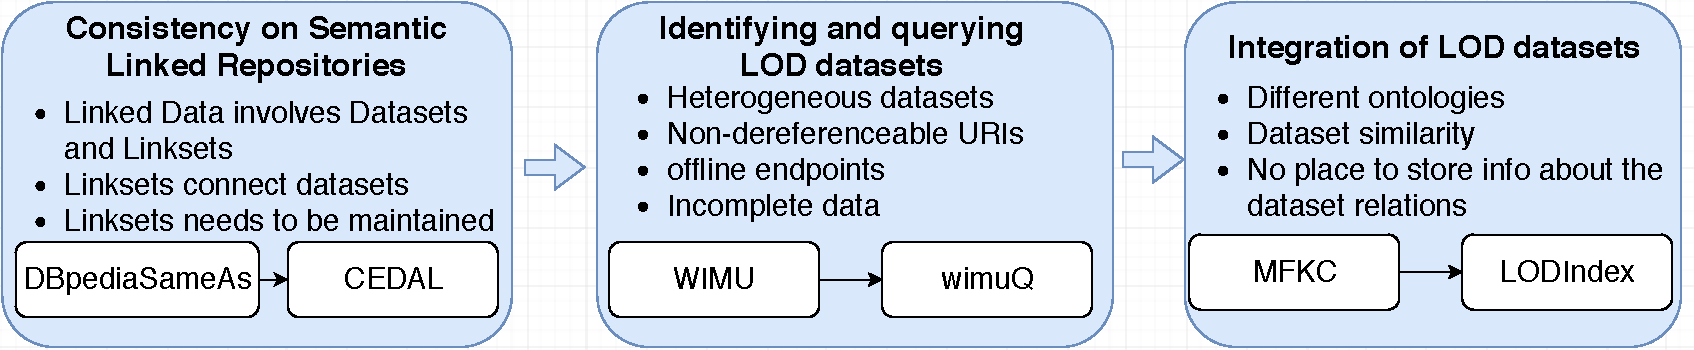
\includegraphics[width=1.0\linewidth]{sections/img/ThesisContribPic.pdf}
%\caption{Contributions of this thesis.}
%\label{fig:contributions}
%\end{figure} 

%The contributions of this thesis can also be visualized in the Linked Data Life-cycle \cite{AUE+11} (a simplification in three steps depicted in \cref{fig:lifecycle}). In which the works DBpediaSameAs~\cite{valdestilhasdbpediasameas} and CEDAL \cite{valdestilhas2017cedal} are related to the \textbf{Classification}, \textbf{Evolution/Repair} and \textbf{Quality}. The works WIMU \cite{valdestilhas2018my}, wimuQ \cite{ValdestilhasKcap}, MFKC  \cite{valdestilhas2017high} and ReLOD \cite{valdestilhas2019ReLOD} are related to \textbf{Interlinking}, \textbf{Storage} and \textbf{Search/Browsing/Exploration}.

\begin{figure}[htb] 
\centering
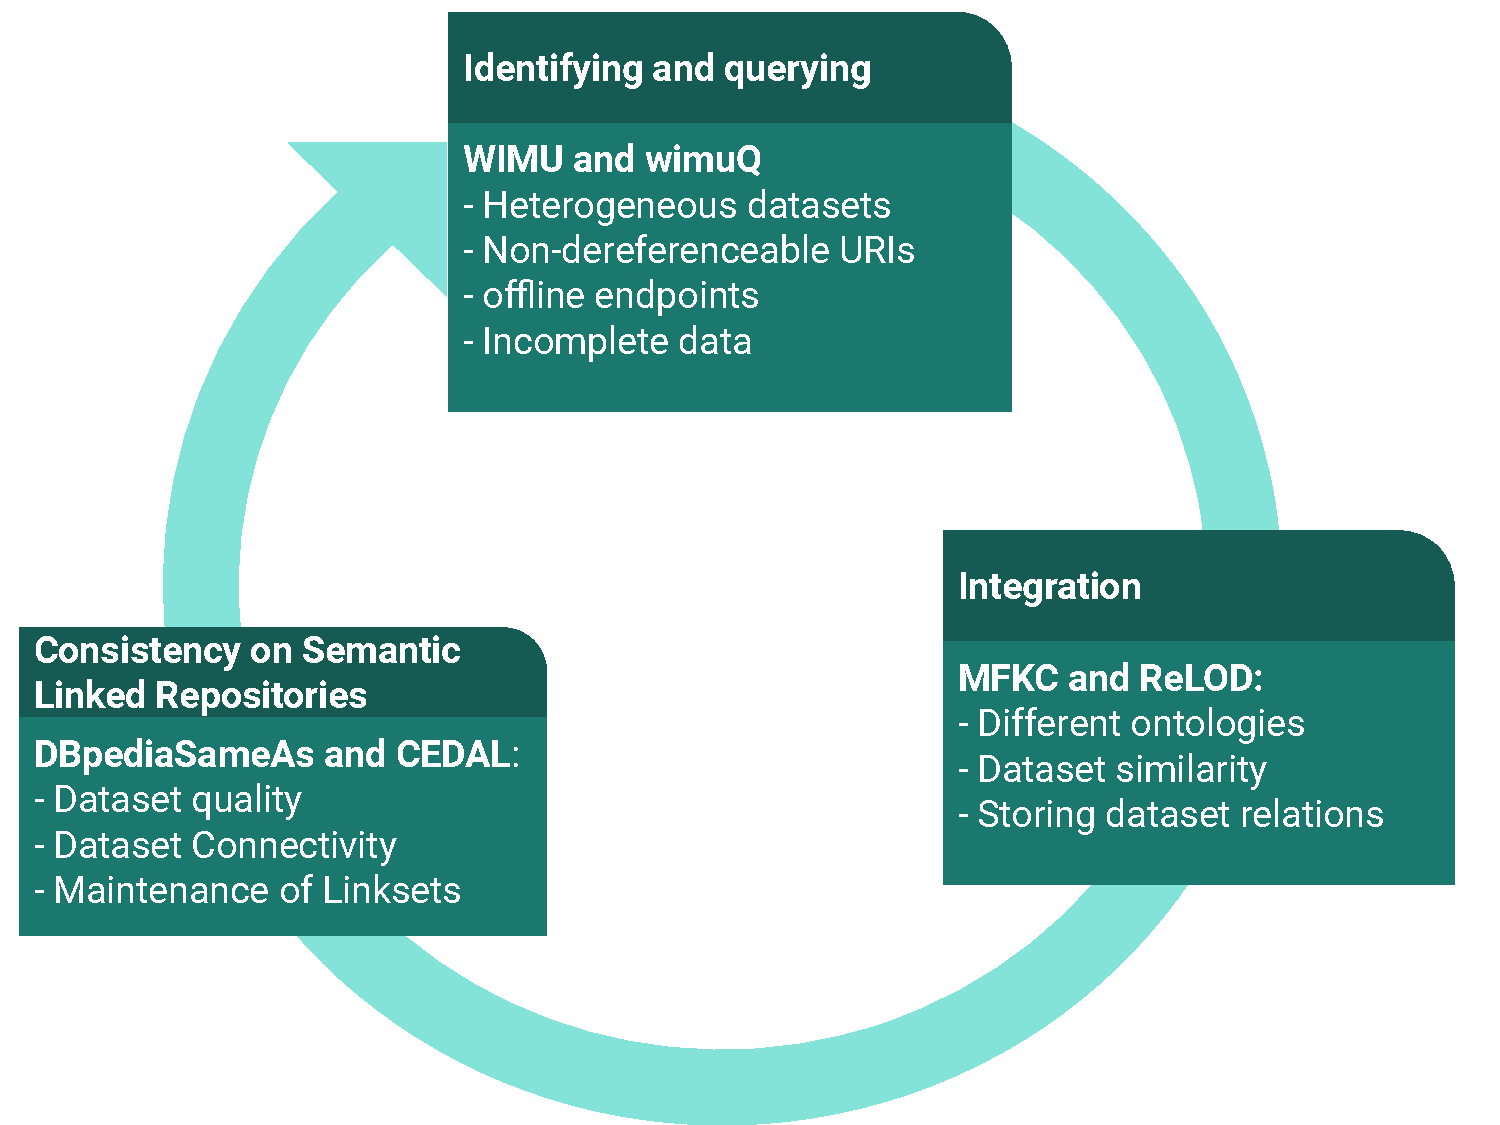
\includegraphics[width=1.0\linewidth]{sections/img/lifeThesis.pdf}
\caption{Life-cycle of contributions.}
\label{fig:lifecycle}
\end{figure} 

\begin{enumerate}
    %WIMU
    \item With WIMU\cite{valdestilhas2018my} we provide a regularly updated database index of more than 660K datasets from LODStats and LOD Laundromat, an efficient, low cost and scalable service on the web that shows which dataset most likely defines a URI and various statistics of datasets indexed from LODStats and LOD Laundromat.
    
    %wimuT
    \item With wimuQ\cite{ValdestilhasKcap} we present a hybrid SPARQL query processing engine which is able to retrieve results from 559 active SPARQL endpoints (with a total of 163.23 billion triples) and 668,166 datasets (with a total of 58.49 billion triples) from LOD Stats and LOD Laudromat. Thus, to the best of our knowledge, WimuQ is the first federated SPARQL query processing engine that executes SPARQL queries over a net total of 221.7 billion triples. As part of WimuQ, we present a low-cost API dubbed \emph{SPARQL-a-lot} to execute SPARQL queries over LOD-a-lot~\cite{fernandez2017lod}, a 300 GB HDT file of the LOD cloud. For the first time, to the best of our knowledge, we make use of the Concise Bounded Descriptions (CBDs) to execute federate SPARQL queries. We also make use of the WIMU index ~\cite{valdestilhas2018my} to intelligently select the capable (also called relevant) \cite{hibiscus2014} data sources pertaining to the given SPARQL query. We evaluated our integrated query engine on two real-data federated SPARQL querying benchmarks \emph{LargeRDFBench} \cite{largerdfbench2017},\emph{FedBench} \cite{fedbench2011} and one non-federated real data SPARQL benchmark selected from \emph{FEASIBLE} \cite{feasible2015} benchmarks generation framework.
    
    %DBpediaSameAs
    \item With DBpediaSameAs\cite{valdestilhas2015dbpediasameas} it was described an approach for the mitigation of the identifier heterogeneity problem and implement a prototype where the user is able to evaluate existing links, as well as suggest new links to be rated. Together with the ability to generate statistics about good and bad links which, brings the possibility to have a quality control for the links to DBpedia. Also we define the DBpedia Unique Identifier (DUI), which instead of several transient \qname{owl:sameAs} DBpedia URIs for the same final address, now is possible to have a unique URI from DBpedia. A DUI goes directly to the final address instead of having to process several possible intermediate results.
    
    %CEDAL
    \item We present CEDAL\cite{valdestilhas2017cedal}, a time-efficient algorithm for the detection of erroneous links in large-scale link repositories without computing all closures required by the property axiom. An approach that brings the possibility to track the consistency problems inside link repositories, in which is a scalable algorithm that works well in a parallel and non-parallel mode. Together with a study case applied to a link repository called LinkLion and a new linkset quality measure based on the number of erroneous candidates.
	
	%MFKC
	\item We present MKFC\cite{valdestilhas2017high}, in which is based in two nested filters, (1) First Frequency Filter and (2) Hash Intersection filter, that allow to discard candidates before calculating the actual similarity value, thus giving a considerable performance gain, including the \emph{k similarity filter} that allows detecting whether two strings $s$ and $t$ are similar in a fewer number of steps. We evaluate our approach with respect to its runtime and its scalability with several threshold settings and dataset sizes. Also, we present several parallel implementations of our approach and show that they work well on problems where $|\ds{} \times \dt{}| \geq 10^5$ pairs.
	
	%LODDatasetRelationIndex
    \item We present ReLOD\cite{valdestilhas2019ReLOD}, a method to create a repository to store the similarity between a large number of datasets involving the detection of duplicated datasets and dataset chunks. To this aim, we store those similarities, providing an index to store the relation among them. The similarities processing is based on thee properties and classes of each dataset. We give a similarity score to each dataset pair and also provide an search engine to find similar datasets, classes and properties for a given a given dataset, class or property. We build the index over a total of 668,166 datasets from LOD Stats and LOD Laudromat as well as 559 active SPARQL endpoints. These data sources represent a total of 221.7 billion triples from more than 5 terabytes of information from datasets partially retrieved using the service ``Where is My URI'' (WIMU). Our evaluation on state-of-the-art real-data shows that more than 90\% of datasets from LODLaundromat datasets are not using owl:equivalentProperty and owl:equivalentClass or other way to relate the data, reinforcing the need for a index of relations among LOD datasets.%\todo{Need to finish and add the paper.}
    
\end{enumerate}

\section{Chapter overview}
\begin{description}
    \item[\textbf{Chapter \ref{ch:preliminaries}}] introduces the basic concepts and notation that are necessary to understand the rest of this thesis. The notation presented in this chapter is used throughout the thesis.
    \item[\textbf{Chapter \ref{ch:soa}}] discusses the state-of-the-art research work related to this thesis.
    \item[\textbf{Chapter \ref{ch:dbpediaSameAs}}] is based on \cite{valdestilhasdbpediasameas} presenting an approach which improves the quality of Link repositories with a case applied to DBpedia, in which shows an approach for the mitigation of the identifier heterogeneity problem and implement a prototype where the user is able to evaluate existing links, as well as suggest new links to be rated.
    \item[\textbf{Chapter \ref{ch:CEDAL}}] is based on \cite{valdestilhas2017cedal} present an extension of the previous work \cite{valdestilhasdbpediasameas} discussing the consistency of semantic web Linked repositories in a more wide point of view.
    \item[\textbf{Chapter \ref{ch:wimu}}] is based on \cite{valdestilhas2018my} and introduces WIMU, a regularly updated database index of more than 660K datasets from LODStats and LOD Laundromat, an efficient, low cost and scalable service on the web that shows which dataset most likely defines a URI.
    \item[\textbf{Chapter \ref{ch:wimuq}}] is based on \cite{ValdestilhasKcap} and presents a hybrid SPARQL query processing engine which is able to retrieve results from a large number of heterogeneous LOD datasets. The approach is called WimuQ in which is the first federated SPARQL query processing engine that executes SPARQL queries over a net total of 221.7 billion triples.
    \item[\textbf{Chapter \ref{ch:MFKC}}] is based on \cite{valdestilhas2017high} and presents two nested filters, (1) First Frequency Filter and (2) Hash Intersection filter, that allow to discard candidates before calculating the actual similarity value, thus giving a considerable performance gain.
    \item[\textbf{Chapter \ref{ch:lodIndex}}] is based on \cite{valdestilhas2019ReLOD} a method to create a repository to store the similarity between a large number of datasets involving the detection of duplicated datasets and dataset chunks. %\todo{Need to update according to the last version of the paper.}
    \item[Finally, \textbf{Chapter \ref{ch:conclusion}}] concludes this work and proposes some future work in related areas of research.
\end{description}
